\documentclass[11pt,aspectratio=169]{beamer}
\usetheme{Madrid}

% ======================= PACKAGES =======================
\usepackage{graphicx}
\usepackage{booktabs}
\usepackage{adjustbox}
\usepackage{multicol}
\usepackage{amsmath}
\usepackage{amssymb}
\usepackage{tikz}
\usetikzlibrary{arrows,shapes,positioning,shadows,trees}
\usepackage{listings}
\usepackage{xcolor}

% ======================= COLOR DEFINITIONS =======================
% Primary color scheme: Blue/Teal for Digital Finance
\definecolor{dfblue}{RGB}{0,102,204}
\definecolor{dfteal}{RGB}{0,153,153}
\definecolor{dfcyan}{RGB}{51,187,204}
\definecolor{dflightblue}{RGB}{153,204,255}
\definecolor{dflightblue2}{RGB}{173,214,255}
\definecolor{dflightblue3}{RGB}{193,224,255}
\definecolor{dflightblue4}{RGB}{213,234,255}

% Accent colors for finance applications
\definecolor{dfgreen}{RGB}{44, 160, 44}
\definecolor{dfred}{RGB}{214, 39, 40}
\definecolor{dforange}{RGB}{255, 127, 14}
\definecolor{dfgray}{RGB}{127, 127, 127}

% Utility colors
\definecolor{lightgray}{RGB}{240, 240, 240}
\definecolor{midgray}{RGB}{180, 180, 180}
\definecolor{codebg}{RGB}{245, 245, 245}

% ======================= THEME CUSTOMIZATION =======================
% Apply Digital Finance color scheme to Madrid theme
\setbeamercolor{palette primary}{bg=dflightblue3,fg=dfblue}
\setbeamercolor{palette secondary}{bg=dflightblue2,fg=dfblue}
\setbeamercolor{palette tertiary}{bg=dfteal,fg=white}
\setbeamercolor{palette quaternary}{bg=dfblue,fg=white}

\setbeamercolor{structure}{fg=dfblue}
\setbeamercolor{section in toc}{fg=dfblue}
\setbeamercolor{subsection in toc}{fg=dfteal}
\setbeamercolor{title}{fg=dfblue}
\setbeamercolor{frametitle}{fg=dfblue,bg=dflightblue3}
\setbeamercolor{block title}{bg=dflightblue2,fg=dfblue}
\setbeamercolor{block body}{bg=dflightblue4,fg=black}

% Remove navigation symbols for cleaner look
\setbeamertemplate{navigation symbols}{}

% Clean itemize/enumerate
\setbeamertemplate{itemize items}[circle]
\setbeamertemplate{enumerate items}[default]

% Margins for readability
\setbeamersize{text margin left=8mm,text margin right=8mm}

% ======================= LISTINGS CONFIGURATION =======================
% Python code style
\lstdefinestyle{pythonstyle}{
    language=Python,
    basicstyle=\ttfamily\footnotesize,
    keywordstyle=\color{dfblue}\bfseries,
    stringstyle=\color{dforange},
    commentstyle=\color{dfgray}\itshape,
    numberstyle=\tiny\color{dfgray},
    numbers=left,
    numbersep=5pt,
    backgroundcolor=\color{codebg},
    showspaces=false,
    showstringspaces=false,
    showtabs=false,
    frame=single,
    rulecolor=\color{midgray},
    tabsize=4,
    captionpos=b,
    breaklines=true,
    breakatwhitespace=false,
    escapeinside={(*@}{@*)},
    xleftmargin=10pt,
    xrightmargin=10pt
}

% Solidity code style
\lstdefinestyle{soliditystyle}{
    language=Java, % closest approximation
    basicstyle=\ttfamily\footnotesize,
    keywordstyle=\color{dfteal}\bfseries,
    stringstyle=\color{dforange},
    commentstyle=\color{dfgray}\itshape,
    numberstyle=\tiny\color{dfgray},
    numbers=left,
    numbersep=5pt,
    backgroundcolor=\color{codebg},
    showspaces=false,
    showstringspaces=false,
    showtabs=false,
    frame=single,
    rulecolor=\color{midgray},
    tabsize=2,
    captionpos=b,
    breaklines=true,
    breakatwhitespace=false,
    escapeinside={(*@}{@*)},
    xleftmargin=10pt,
    xrightmargin=10pt,
    morekeywords={pragma, contract, function, returns, public, private, view, pure, payable, address, uint256, mapping, event, modifier}
}

% Inline code command
\newcommand{\code}[1]{\texttt{\color{dfblue}#1}}

% ======================= CUSTOM COMMANDS =======================
% Bottom annotation (Madrid-style)
\newcommand{\bottomnote}[1]{%
\vfill
\vspace{-2mm}
\textcolor{dflightblue2}{\rule{\textwidth}{0.4pt}}
\vspace{1mm}
\footnotesize
\textbf{#1}
}

% Compact list spacing
\newcommand{\compactlist}{%
\setlength{\itemsep}{0pt}%
\setlength{\parskip}{0pt}%
\setlength{\parsep}{0pt}%
}

% Chart placeholder
\newcommand{\chartplaceholder}[2][5cm]{%
\begin{center}
\begin{adjustbox}{max width=0.95\textwidth, max height=#1}
\framebox[\textwidth][c]{%
\rule{0pt}{#1}%
\textcolor{midgray}{[#2]}%
}
\end{adjustbox}
\end{center}
}

% ======================= FINANCE NOTATION MACROS =======================
% Probability and statistics
\newcommand{\E}{\mathbb{E}} % Expected value
\newcommand{\Var}{\mathrm{Var}} % Variance
\newcommand{\Cov}{\mathrm{Cov}} % Covariance
\newcommand{\Prob}{\mathbb{P}} % Probability

% Distributions
\newcommand{\Normal}{\mathcal{N}} % Normal distribution
\newcommand{\Uniform}{\mathcal{U}} % Uniform distribution

% Returns and prices
\newcommand{\Ret}{R} % Return
\newcommand{\LogRet}{r} % Log return
\newcommand{\Price}{S} % Price/Stock price
\newcommand{\Strike}{K} % Strike price

% Options and derivatives
\newcommand{\CallPrice}{C} % Call option price
\newcommand{\PutPrice}{P} % Put option price
\newcommand{\Greeks}[1]{\mathit{#1}} % Greek letters

% Risk measures
\newcommand{\VaR}{\mathrm{VaR}} % Value at Risk
\newcommand{\CVaR}{\mathrm{CVaR}} % Conditional VaR
\newcommand{\Sharpe}{\mathrm{SR}} % Sharpe Ratio

% Time series
\newcommand{\AR}{\mathrm{AR}} % Autoregressive
\newcommand{\MA}{\mathrm{MA}} % Moving average
\newcommand{\GARCH}{\mathrm{GARCH}} % GARCH

% Blockchain/Crypto
\newcommand{\Hash}{\mathrm{Hash}} % Hash function
\newcommand{\Block}{\mathcal{B}} % Block
\newcommand{\Chain}{\mathcal{C}} % Chain

% Real numbers, integers
\newcommand{\R}{\mathbb{R}}
\newcommand{\Z}{\mathbb{Z}}
\newcommand{\N}{\mathbb{N}}

% ======================= TIKZ STYLES =======================
% Styles for finance-related diagrams
\tikzstyle{process} = [rectangle, minimum width=3cm, minimum height=1cm, text centered, draw=dfblue, fill=dflightblue4, thick]
\tikzstyle{decision} = [diamond, minimum width=3cm, minimum height=1cm, text centered, draw=dfteal, fill=dflightblue4, thick]
\tikzstyle{arrow} = [thick,->,>=stealth,color=dfblue]
\tikzstyle{blockchain} = [rectangle, rounded corners, minimum width=2.5cm, minimum height=1cm, text centered, draw=dfteal, fill=dflightblue3, thick]
\tikzstyle{transaction} = [circle, minimum size=0.8cm, text centered, draw=dforange, fill=dflightblue4, thick]

% ======================= FOOTER TEMPLATE =======================
\setbeamertemplate{footline}{
    \hbox{\begin{beamercolorbox}[wd=\paperwidth,ht=2.5ex,dp=1ex,leftskip=.5em,rightskip=.5em]{author in head/foot}
    \tiny
    \textbf{Digital Finance} \hfill
    Joerg Osterrieder \hfill
    \insertdate \hfill
    Page \insertframenumber{} / \inserttotalframenumber
    \end{beamercolorbox}}
}

% ======================= SECTION DIVIDER TEMPLATE =======================
\AtBeginSection[]{
\begin{frame}[plain]
\vfill
\centering
\begin{beamercolorbox}[sep=12pt,center]{title}
\usebeamerfont{title}\LARGE\insertsection\par
\end{beamercolorbox}
\vfill
\end{frame}
}


% ======================= DOCUMENT INFO =======================
\title{Topic 2.3: Data-Driven Finance}
\subtitle{Lending, Scoring, and Algorithmic Decision-Making}
\author{Joerg Osterrieder}
\institute{Digital Finance}
\date{2025}

\begin{document}

% ============================================================================
% SLIDE 1: Title
% ============================================================================
\begin{frame}
\titlepage
\end{frame}

% ============================================================================
% SLIDE 2: Learning Objectives
% ============================================================================
\begin{frame}{Learning Objectives}
\begin{block}{By the end of this topic, you will be able to:}
\begin{enumerate}
\item \textbf{Explain} how traditional credit scoring (FICO) works and its limitations
\item \textbf{Identify} types of alternative data used in modern credit decisions
\item \textbf{Compare} traditional statistical models with machine learning approaches
\item \textbf{Recognize} sources of algorithmic bias in lending models
\item \textbf{Understand} explainability requirements and regulatory frameworks
\item \textbf{Analyze} how FinTech lenders use data advantages to compete
\end{enumerate}
\end{block}

\vspace{3mm}
\textbf{Key Competency}: Explain how alternative data and ML models change credit decisions, and identify potential sources of algorithmic bias.

\bottomnote{Hands-on: Notebook NB04 -- Building a Credit Scoring Model}
\end{frame}

% ============================================================================
% SLIDE 3: Prerequisites - What is Credit?
% ============================================================================
\begin{frame}{Prerequisites: Understanding Credit}
\begin{columns}[T]
\begin{column}{0.5\textwidth}
\textbf{What is Credit?}
\begin{itemize}
\item A contractual agreement where a borrower receives something of value now
\item Promises to repay the lender at a later date
\item Usually with interest (the ``price'' of borrowing)
\end{itemize}

\vspace{3mm}
\textbf{Types of Consumer Credit:}
\begin{itemize}
\item \textcolor{dfblue}{Revolving}: Credit cards, lines of credit
\item \textcolor{dfteal}{Installment}: Mortgages, auto loans, personal loans
\item \textcolor{dforange}{Point-of-sale}: Buy Now Pay Later (BNPL)
\end{itemize}
\end{column}
\begin{column}{0.5\textwidth}
\begin{block}{Why Credit Matters}
\begin{itemize}
\item Enables major purchases (home, car, education)
\item Smooths consumption over time
\item Fuels economic growth
\item Access to credit = economic opportunity
\end{itemize}
\end{block}

\vspace{2mm}
\begin{alertblock}{The Core Problem}
How does a lender know if a borrower will repay?
\end{alertblock}
\end{column}
\end{columns}
\end{frame}

% ============================================================================
% SLIDE 4: Prerequisites - Credit Risk Basics
% ============================================================================
\begin{frame}{Prerequisites: Credit Risk Fundamentals}
\begin{columns}[T]
\begin{column}{0.5\textwidth}
\textbf{What is Credit Risk?}
\begin{itemize}
\item The risk that a borrower will \textbf{default}---fail to repay as agreed
\item Lenders must estimate this risk \textit{before} lending
\item Higher risk = higher interest rate (risk premium)
\end{itemize}

\vspace{3mm}
\textbf{Key Terms:}
\begin{itemize}
\item \textcolor{dfblue}{Default}: Failure to make required payments
\item \textcolor{dfblue}{Delinquency}: Late payment (30, 60, 90 days)
\item \textcolor{dfblue}{Principal}: Amount borrowed
\item \textcolor{dfblue}{Interest}: Cost of borrowing
\end{itemize}
\end{column}
\begin{column}{0.5\textwidth}
\begin{block}{Credit Scoring Purpose}
A \textbf{credit score} estimates the \textbf{probability} that a borrower will default.
\end{block}

\vspace{3mm}
\textbf{What Lenders Want to Know:}
\begin{enumerate}
\item Will this person repay? (Willingness)
\item Can this person repay? (Capacity)
\item What happens if they don't? (Collateral)
\end{enumerate}

\vspace{3mm}
\textit{Credit scoring automates these judgments using data.}
\end{column}
\end{columns}
\end{frame}

% ============================================================================
% SLIDE 5: Traditional Credit Scoring - FICO Introduction
% ============================================================================
\begin{frame}{Traditional Credit Scoring: The FICO Score}
\begin{columns}[T]
\begin{column}{0.5\textwidth}
\textbf{What is a FICO Score?}
\begin{itemize}
\item Created by Fair Isaac Corporation (1989)
\item Most widely used credit score in the US
\item Score range: \textbf{300--850}
\item Higher score = lower predicted risk
\end{itemize}

\vspace{3mm}
\textbf{Score Categories:}
\begin{itemize}
\item 800--850: Exceptional
\item 740--799: Very Good
\item \textcolor{dfgreen}{670--739: Good (``Prime'')}
\item \textcolor{dforange}{580--669: Fair}
\item \textcolor{dfred}{300--579: Poor (``Subprime'')}
\end{itemize}
\end{column}
\begin{column}{0.5\textwidth}
\begin{block}{How FICO is Used}
\begin{itemize}
\item Loan approval decisions
\item Interest rate determination
\item Credit limit setting
\item Insurance pricing
\item Rental applications
\item Employment screening
\end{itemize}
\end{block}

\vspace{2mm}
\textbf{Impact}: Your FICO score affects the cost of nearly every major financial decision you make.
\end{column}
\end{columns}
\end{frame}

% ============================================================================
% SLIDE 6: FICO Components
% ============================================================================
\begin{frame}{FICO Score Components: What Matters Most}
\begin{columns}[T]
\begin{column}{0.5\textwidth}
\textbf{FICO Score Breakdown:}
\begin{itemize}
\item \textcolor{dfblue}{\textbf{Payment History: 35\%}}\\
On-time vs. late payments
\item \textcolor{dfteal}{\textbf{Amounts Owed: 30\%}}\\
Credit utilization ratio
\item \textcolor{dfgreen}{\textbf{Length of Credit History: 15\%}}\\
Average age of accounts
\item \textcolor{dforange}{\textbf{New Credit: 10\%}}\\
Recent inquiries and new accounts
\item \textcolor{dfred}{\textbf{Credit Mix: 10\%}}\\
Variety of account types
\end{itemize}
\end{column}
\begin{column}{0.5\textwidth}
\begin{center}
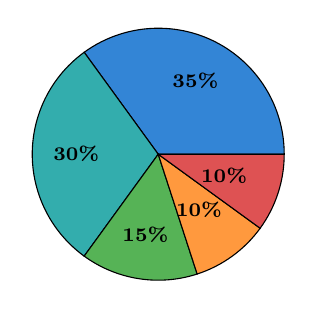
\begin{tikzpicture}[scale=0.8]
% Pie chart segments
\draw[fill=dfblue!80] (0,0) -- (0:2) arc (0:126:2) -- cycle;
\draw[fill=dfteal!80] (0,0) -- (126:2) arc (126:234:2) -- cycle;
\draw[fill=dfgreen!80] (0,0) -- (234:2) arc (234:288:2) -- cycle;
\draw[fill=dforange!80] (0,0) -- (288:2) arc (288:324:2) -- cycle;
\draw[fill=dfred!80] (0,0) -- (324:2) arc (324:360:2) -- cycle;

% Labels
\node[font=\scriptsize] at (63:1.3) {\textbf{35\%}};
\node[font=\scriptsize] at (180:1.3) {\textbf{30\%}};
\node[font=\scriptsize] at (261:1.3) {\textbf{15\%}};
\node[font=\scriptsize] at (306:1.1) {\textbf{10\%}};
\node[font=\scriptsize] at (342:1.1) {\textbf{10\%}};
\end{tikzpicture}
\end{center}

\vspace{2mm}
\textbf{Key Insight}: 65\% of your score depends on payment behavior and debt levels.
\end{column}
\end{columns}
\end{frame}

% ============================================================================
% SLIDE 7: FICO Limitations
% ============================================================================
\begin{frame}{FICO Limitations: Who Gets Left Behind?}
\begin{columns}[T]
\begin{column}{0.5\textwidth}
\begin{alertblock}{Critical Limitations}
\begin{itemize}
\item \textbf{45 million ``credit invisible''}:\\
No credit score at all
\item \textbf{Thin file problem}:\\
Too little history to score
\item \textbf{Stale data}:\\
Updated only monthly
\item \textbf{No income data}:\\
Only credit behavior
\item \textbf{Backward-looking}:\\
Past predicts future?
\end{itemize}
\end{alertblock}
\end{column}
\begin{column}{0.5\textwidth}
\textbf{Who is Credit Invisible?}
\begin{itemize}
\item Young adults / students
\item Recent immigrants
\item People who use cash
\item Divorced individuals (shared accounts)
\item Those recovering from bankruptcy
\end{itemize}

\vspace{3mm}
\begin{block}{The Opportunity}
Millions of \textbf{creditworthy} people are excluded by traditional scores---not because they can't repay, but because they lack traditional credit history.
\end{block}
\end{column}
\end{columns}

\vspace{2mm}
\textbf{FinTech insight}: Alternative data can identify creditworthy thin-file borrowers.
\end{frame}

% ============================================================================
% SLIDE 8: Credit Bureaus
% ============================================================================
\begin{frame}{The Credit Bureau System}
\begin{columns}[T]
\begin{column}{0.55\textwidth}
\textbf{Three Major Credit Bureaus (US):}
\begin{enumerate}
\item \textbf{Equifax} (founded 1899)
\item \textbf{Experian} (founded 1996, UK origin)
\item \textbf{TransUnion} (founded 1968)
\end{enumerate}

\vspace{3mm}
\textbf{What Bureaus Do:}
\begin{itemize}
\item Collect credit data from lenders
\item Maintain individual credit files
\item Sell credit reports to lenders
\item Calculate credit scores
\item Provide data for FICO models
\end{itemize}
\end{column}
\begin{column}{0.45\textwidth}
\begin{block}{Bureau Data Sources}
\begin{itemize}
\item Banks and credit unions
\item Credit card companies
\item Mortgage lenders
\item Auto lenders
\item Collection agencies
\item Public records (bankruptcies)
\end{itemize}
\end{block}

\vspace{2mm}
\textbf{Key Point}: Bureaus are \textit{information intermediaries}---they don't make lending decisions, but provide the data infrastructure.
\end{column}
\end{columns}
\end{frame}

% ============================================================================
% SLIDE 9: Alternative Data Introduction
% ============================================================================
\begin{frame}{Alternative Data: Beyond the Credit Bureau}
\begin{block}{Definition}
\textbf{Alternative data}: Information not found in traditional credit bureau reports that can predict creditworthiness.
\end{block}

\vspace{3mm}
\begin{center}
\begin{tabular}{p{3.2cm}p{4cm}p{3.5cm}}
\toprule
\textbf{Data Type} & \textbf{Signal} & \textbf{Used By} \\
\midrule
Bank transactions & Cash flow, spending patterns & Plaid, Petal \\
Rent payments & Payment reliability & Experian Boost \\
Utility bills & Consistent payments & FICO XD \\
Employment/payroll & Income stability & Argyle, Pinwheel \\
Social media & Network, behavior & (controversial) \\
Device/browser data & Fraud signals & Socure, Sardine \\
Education history & Future earning potential & Upstart \\
Shopping behavior & Financial responsibility & Affirm \\
\bottomrule
\end{tabular}
\end{center}
\end{frame}

% ============================================================================
% SLIDE 10: Alternative Data Examples
% ============================================================================
\begin{frame}{Alternative Data: Detailed Examples}
\begin{columns}[T]
\begin{column}{0.5\textwidth}
\textbf{Bank Transaction Data:}
\begin{itemize}
\item Income consistency and volatility
\item Rent-to-income ratio
\item Overdraft frequency
\item Savings patterns
\item Recurring bill payments
\end{itemize}

\vspace{3mm}
\textbf{Employment Data:}
\begin{itemize}
\item Job tenure
\item Salary verification
\item Industry/occupation
\item Employer stability
\end{itemize}
\end{column}
\begin{column}{0.5\textwidth}
\textbf{Behavioral Data:}
\begin{itemize}
\item Time of day applying
\item Device type and browser
\item How form fields are completed
\item Typing speed and patterns
\end{itemize}

\vspace{3mm}
\begin{alertblock}{Privacy Tension}
More data $\rightarrow$ better predictions\\
More data $\rightarrow$ privacy concerns

\vspace{2mm}
\textit{Where should the line be drawn?}
\end{alertblock}
\end{column}
\end{columns}
\end{frame}

% ============================================================================
% SLIDE 11: Traditional vs ML Models
% ============================================================================
\begin{frame}{Machine Learning in Credit: How It Works}
\begin{columns}[T]
\begin{column}{0.55\textwidth}
\textbf{Traditional (Logistic Regression):}
\begin{itemize}
\item Linear combinations of features
\item Easy to interpret (coefficients)
\item Required by some regulations
\item Limited to known relationships
\end{itemize}

\vspace{2mm}
\textbf{ML Models (XGBoost, Neural Nets):}
\begin{itemize}
\item Non-linear relationships
\item Feature interactions automatic
\item Higher predictive accuracy
\item ``Black box'' interpretability issues
\end{itemize}
\end{column}
\begin{column}{0.45\textwidth}
\begin{block}{Accuracy Improvement}
ML models can improve:
\begin{itemize}
\item Default prediction: \textcolor{dfgreen}{15--25\%}
\item Approval rates: \textcolor{dfgreen}{10--20\% more}
\item Loss rates: \textcolor{dfgreen}{10--15\% lower}
\end{itemize}
\vspace{2mm}
\textbf{Upstart claim}: 27\% more approvals at same loss rate
\end{block}
\end{column}
\end{columns}

\vspace{3mm}
\textbf{Key Trade-off}: Accuracy vs. Explainability
\end{frame}

% ============================================================================
% SLIDE 12: Logistic Regression Explained
% ============================================================================
\begin{frame}{Logistic Regression: The Traditional Workhorse}
\begin{columns}[T]
\begin{column}{0.55\textwidth}
\textbf{How It Works:}
\begin{itemize}
\item Predicts probability of default: $P(\text{default})$
\item Combines features linearly
\item Applies sigmoid function to bound 0--1
\end{itemize}

\vspace{2mm}
\textbf{Mathematical Form:}
\[
P(\text{default}) = \frac{1}{1 + e^{-(\beta_0 + \beta_1 x_1 + \beta_2 x_2 + ...)}}
\]

\vspace{2mm}
\textbf{Interpreting Coefficients:}
\begin{itemize}
\item $\beta > 0$: Higher value $\rightarrow$ more risk
\item $\beta < 0$: Higher value $\rightarrow$ less risk
\item Magnitude indicates strength
\end{itemize}
\end{column}
\begin{column}{0.45\textwidth}
\begin{block}{Why Regulators Like It}
\begin{itemize}
\item Each feature's impact is clear
\item Can explain: ``You were declined because of high debt-to-income ratio''
\item Easy to audit for bias
\item Stable and well-understood
\end{itemize}
\end{block}

\vspace{2mm}
\textbf{Example Coefficients:}
\begin{itemize}
\item Debt-to-income: $+0.8$
\item Payment history: $-1.2$
\item Credit age: $-0.3$
\end{itemize}
\end{column}
\end{columns}
\end{frame}

% ============================================================================
% SLIDE 13: Credit Scoring Pipeline
% ============================================================================
\begin{frame}{Credit Scoring Pipeline}
\begin{center}
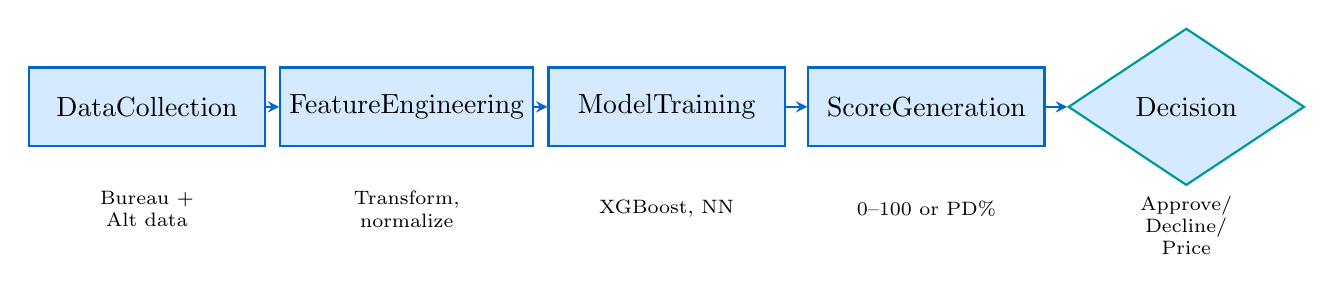
\begin{tikzpicture}[node distance=1.8cm]
% Pipeline nodes
\node (data) [process] {Data\\Collection};
\node (feature) [process, right of=data, xshift=1.5cm] {Feature\\Engineering};
\node (model) [process, right of=feature, xshift=1.5cm] {Model\\Training};
\node (score) [process, right of=model, xshift=1.5cm] {Score\\Generation};
\node (decision) [decision, right of=score, xshift=1.5cm] {Decision};

% Arrows
\draw[arrow] (data) -- (feature);
\draw[arrow] (feature) -- (model);
\draw[arrow] (model) -- (score);
\draw[arrow] (score) -- (decision);

% Labels below
\node[below of=data, yshift=0.5cm, font=\scriptsize, text width=2cm, align=center] {Bureau + Alt data};
\node[below of=feature, yshift=0.5cm, font=\scriptsize, text width=2cm, align=center] {Transform, normalize};
\node[below of=model, yshift=0.5cm, font=\scriptsize, text width=2cm, align=center] {XGBoost, NN};
\node[below of=score, yshift=0.5cm, font=\scriptsize, text width=2cm, align=center] {0--100 or PD\%};
\node[below of=decision, yshift=0.3cm, font=\scriptsize, text width=2cm, align=center] {Approve/\\Decline/\\Price};
\end{tikzpicture}
\end{center}

\vspace{3mm}
\begin{block}{Key Decisions at Each Stage}
\begin{itemize}
\item \textbf{Data}: What sources? Privacy implications?
\item \textbf{Features}: What transformations? What to exclude?
\item \textbf{Model}: Accuracy vs. interpretability trade-off?
\item \textbf{Decision}: Cutoffs, pricing tiers, human review thresholds?
\end{itemize}
\end{block}
\end{frame}

% ============================================================================
% SLIDE 14: Feature Engineering
% ============================================================================
\begin{frame}[fragile]{Feature Engineering: Transforming Raw Data}
\begin{lstlisting}[style=pythonstyle, basicstyle=\ttfamily\scriptsize]
# Raw transaction data
transactions = [
    {"date": "2024-01-15", "amount": -1200, "category": "rent"},
    {"date": "2024-01-14", "amount": 3500, "category": "payroll"},
    {"date": "2024-01-10", "amount": -45, "category": "food"},
    ...
]

# Engineered features
features = {
    "avg_monthly_income": 3500,
    "income_volatility": 0.05,      # Low = stable
    "rent_to_income_ratio": 0.34,   # Below 0.4 = good
    "days_since_overdraft": 180,    # Higher = better
    "recurring_payment_count": 12,  # Shows organization
    "gambling_transaction_flag": 0, # Red flag if present
}
\end{lstlisting}

\vspace{2mm}
\textbf{Key insight}: Raw data becomes predictive through thoughtful engineering.

\bottomnote{Notebook NB04: Engineer features from transaction data and see how they affect model predictions}
\end{frame}

% ============================================================================
% SLIDE 15: Model Evaluation Metrics
% ============================================================================
\begin{frame}{Model Evaluation: How Good is the Model?}
\begin{columns}[T]
\begin{column}{0.5\textwidth}
\textbf{Key Metrics:}

\vspace{2mm}
\textbf{1. AUC (Area Under ROC Curve):}
\begin{itemize}
\item Measures ranking ability
\item 0.5 = random, 1.0 = perfect
\item Industry standard: 0.70--0.80
\end{itemize}

\vspace{2mm}
\textbf{2. Gini Coefficient:}
\begin{itemize}
\item Gini = 2 $\times$ AUC $-$ 1
\item Measures separation power
\item Gini of 0.50 = AUC of 0.75
\end{itemize}
\end{column}
\begin{column}{0.5\textwidth}
\textbf{3. Calibration:}
\begin{itemize}
\item Do predicted probabilities match reality?
\item If model says 20\% default, do 20\% actually default?
\item Critical for pricing decisions
\end{itemize}

\vspace{2mm}
\begin{block}{Why Both Matter}
\begin{itemize}
\item \textbf{AUC}: Can we \textit{rank} borrowers correctly?
\item \textbf{Calibration}: Are probabilities \textit{accurate}?
\end{itemize}

A model can rank well but be poorly calibrated!
\end{block}
\end{column}
\end{columns}
\end{frame}

% ============================================================================
% SLIDE 16: Algorithmic Bias Introduction
% ============================================================================
\begin{frame}{Algorithmic Bias: The Dark Side}
\begin{columns}[T]
\begin{column}{0.5\textwidth}
\textbf{Sources of Bias:}
\begin{enumerate}
\item \textbf{Historical data}:\\
Past discrimination encoded
\item \textbf{Proxy variables}:\\
ZIP code $\approx$ race
\item \textbf{Sample bias}:\\
Training on existing customers only
\item \textbf{Feature selection}:\\
Human choices embedded
\end{enumerate}

\vspace{2mm}
\textbf{Legal Framework (US):}
\begin{itemize}
\item ECOA: No discrimination by protected class
\item Disparate impact: Unintentional bias illegal
\item Adverse action notices: Must explain denials
\end{itemize}
\end{column}
\begin{column}{0.5\textwidth}
\begin{alertblock}{Apple Card Investigation (2019)}
Same household, shared finances:\\
\textbf{Husband}: \$20,000 limit\\
\textbf{Wife}: \$200 limit\\
\vspace{2mm}
Algorithm couldn't explain why.\\
NY DFS investigation followed.
\end{alertblock}

\begin{block}{Testing for Bias}
\begin{itemize}
\item Demographic parity
\item Equal opportunity
\item Calibration across groups
\end{itemize}
\end{block}
\end{column}
\end{columns}
\end{frame}

% ============================================================================
% SLIDE 17: Disparate Impact
% ============================================================================
\begin{frame}{Disparate Impact: Unintentional Discrimination}
\begin{columns}[T]
\begin{column}{0.5\textwidth}
\textbf{What is Disparate Impact?}
\begin{itemize}
\item Policies that \textit{appear} neutral
\item But disproportionately harm protected groups
\item Even without discriminatory \textit{intent}
\item Still illegal under fair lending laws
\end{itemize}

\vspace{3mm}
\textbf{The Four-Fifths Rule:}
\begin{itemize}
\item Selection rate for protected group
\item Should be $\geq$ 80\% of majority group
\item Example: If 50\% of white applicants approved, need $\geq$ 40\% minority approval
\end{itemize}
\end{column}
\begin{column}{0.5\textwidth}
\begin{alertblock}{Proxy Variables Problem}
Features that correlate with protected characteristics:
\begin{itemize}
\item ZIP code $\rightarrow$ race
\item Name patterns $\rightarrow$ ethnicity
\item School attended $\rightarrow$ socioeconomic status
\end{itemize}

\vspace{2mm}
Even if race isn't a feature, the model may learn to discriminate through proxies.
\end{alertblock}
\end{column}
\end{columns}

\vspace{3mm}
\textbf{Key point}: Good intentions don't prevent illegal outcomes.
\end{frame}

% ============================================================================
% SLIDE 18: Reject Inference Problem
% ============================================================================
\begin{frame}{The Reject Inference Problem}
\begin{columns}[T]
\begin{column}{0.55\textwidth}
\textbf{The Problem:}
\begin{itemize}
\item We only observe outcomes for \textit{approved} loans
\item What about people we rejected?
\item Their true default risk is unknown
\item This creates \textbf{selection bias}
\end{itemize}

\vspace{3mm}
\textbf{Example:}
\begin{itemize}
\item Train model on approved loans only
\item Model learns: ``low scores = bad''
\item But some low-score rejects might have repaid!
\item Model becomes overly conservative
\end{itemize}
\end{column}
\begin{column}{0.45\textwidth}
\begin{block}{Solutions (Imperfect)}
\begin{enumerate}
\item \textbf{Clean sample}: Use only approved (biased)
\item \textbf{Through-the-door}: Try to include all
\item \textbf{Reject inference}: Impute outcomes
\item \textbf{Champion/Challenger}: Randomly approve some rejects
\end{enumerate}
\end{block}

\vspace{2mm}
\textbf{Trade-off}: All approaches involve assumptions about unknown data.
\end{column}
\end{columns}
\end{frame}

% ============================================================================
% SLIDE 19: Explainability Challenge
% ============================================================================
\begin{frame}{Explainability: The Interpretability Challenge}
\begin{columns}[T]
\begin{column}{0.5\textwidth}
\textbf{Why Explainability Matters:}
\begin{itemize}
\item Regulatory requirement (adverse action)
\item Consumer trust and understanding
\item Model debugging and validation
\item Fairness auditing
\end{itemize}

\vspace{2mm}
\textbf{Explainability Techniques:}
\begin{itemize}
\item \textbf{SHAP values}: Feature contributions
\item \textbf{LIME}: Local interpretable explanations
\item \textbf{Feature importance}: Global rankings
\item \textbf{Partial dependence}: Effect of single features
\end{itemize}
\end{column}
\begin{column}{0.5\textwidth}
\begin{block}{Adverse Action Example}
``Your application was declined because:
\begin{enumerate}
\item High credit utilization (78\%)
\item Short credit history (2 years)
\item Recent late payment (30+ days)
\item High number of inquiries (6)
\end{enumerate}''
\end{block}
\vspace{2mm}
\textbf{Challenge}: ML models may not map cleanly to these simple reasons.
\end{column}
\end{columns}
\end{frame}

% ============================================================================
% SLIDE 20: SHAP Values Explained
% ============================================================================
\begin{frame}{SHAP Values: Explaining Individual Predictions}
\begin{columns}[T]
\begin{column}{0.55\textwidth}
\textbf{What is SHAP?}
\begin{itemize}
\item \textbf{SH}apley \textbf{A}dditive ex\textbf{P}lanations
\item Based on game theory (Shapley values)
\item Assigns each feature a contribution to the prediction
\item Contributions sum to the prediction
\end{itemize}

\vspace{3mm}
\textbf{Example Output:}
\begin{itemize}
\item Base score: 650
\item Income (+40): High income helps
\item Debt-to-income (-60): High ratio hurts
\item Payment history (+25): Good history
\item \textbf{Final score: 655}
\end{itemize}
\end{column}
\begin{column}{0.45\textwidth}
\begin{block}{Why SHAP for Credit}
\begin{itemize}
\item Explains \textit{any} model (even neural nets)
\item Consistent and fair allocation
\item Can identify bias sources
\item Regulatory-friendly documentation
\end{itemize}
\end{block}

\vspace{2mm}
\textbf{Limitation}: Computationally expensive for complex models with many features.
\end{column}
\end{columns}
\end{frame}

% ============================================================================
% SLIDE 21: FinTech Lenders Business Models
% ============================================================================
\begin{frame}{FinTech Lenders: Business Models}
\begin{center}
\begin{tabular}{p{2.2cm}p{2.8cm}p{3cm}p{2.5cm}}
\toprule
\textbf{Company} & \textbf{Model} & \textbf{Data Edge} & \textbf{Economics} \\
\midrule
\textbf{Upstart} & AI underwriting & Education, employment & 25\% lower losses \\
\textbf{SoFi} & Member ecosystem & Product usage & Cross-sell \\
\textbf{Affirm} & POS lending & Purchase behavior & Merchant fees \\
\textbf{LendingClub} & Marketplace & Platform data & Origination fees \\
\textbf{Kabbage} & SMB lending & Accounting data & Higher rates \\
\bottomrule
\end{tabular}
\end{center}

\vspace{4mm}
\begin{block}{Key Insight}
FinTech lenders compete on \textbf{data advantage}, not cost of capital.\\
Banks have cheaper funding; FinTechs have better risk selection.
\end{block}
\end{frame}

% ============================================================================
% SLIDE 22: Beyond Credit - Algorithmic Decisions
% ============================================================================
\begin{frame}{Beyond Credit: Algorithmic Decisions in Finance}
\begin{columns}[T]
\begin{column}{0.5\textwidth}
\textbf{Insurance (Insurtech):}
\begin{itemize}
\item Telematics (driving behavior)
\item IoT sensors (home/health)
\item Claims fraud detection
\item Dynamic pricing
\end{itemize}

\vspace{2mm}
\textbf{Investment (Robo-advisors):}
\begin{itemize}
\item Risk profiling algorithms
\item Automated rebalancing
\item Tax-loss harvesting
\item Goal-based allocation
\end{itemize}
\end{column}
\begin{column}{0.5\textwidth}
\textbf{Fraud Detection:}
\begin{itemize}
\item Real-time transaction scoring
\item Behavioral biometrics
\item Device fingerprinting
\item Network analysis
\end{itemize}

\vspace{2mm}
\textbf{AML/KYC:}
\begin{itemize}
\item Identity verification
\item Document analysis (OCR)
\item PEP/sanctions screening
\item Suspicious activity patterns
\end{itemize}
\end{column}
\end{columns}

\vspace{3mm}
\textbf{Common thread}: Data + algorithms replacing human judgment across finance.
\end{frame}

% ============================================================================
% SLIDE 23: The Data Flywheel
% ============================================================================
\begin{frame}{The Data Flywheel}
\begin{center}
\begin{tikzpicture}[node distance=2.5cm]
% Circular nodes
\node (more_data) [blockchain] {More Data};
\node (better_models) [blockchain, right of=more_data, xshift=2cm] {Better Models};
\node (better_decisions) [blockchain, below of=better_models] {Better Decisions};
\node (more_customers) [blockchain, left of=better_decisions, xshift=-2cm] {More Customers};

% Circular arrows
\draw[arrow, bend left=20] (more_data) to (better_models);
\draw[arrow, bend left=20] (better_models) to (better_decisions);
\draw[arrow, bend left=20] (better_decisions) to (more_customers);
\draw[arrow, bend left=20] (more_customers) to (more_data);

% Center label
\node at ($(more_data)!0.5!(better_decisions)$) {\textbf{Data Flywheel}};
\end{tikzpicture}
\end{center}

\vspace{3mm}
\textbf{Implication}: First-mover advantage in data creates compounding moat

\textbf{Challenge}: Incumbents have more historical data; FinTechs have more diverse data
\end{frame}

% ============================================================================
% SLIDE 24: Regulatory Landscape
% ============================================================================
\begin{frame}{Regulatory Landscape for ML in Credit}
\begin{columns}[T]
\begin{column}{0.5\textwidth}
\textbf{US Framework:}
\begin{itemize}
\item \textbf{ECOA}: Equal Credit Opportunity Act---fair lending
\item \textbf{FCRA}: Fair Credit Reporting Act---data accuracy
\item \textbf{CFPB}: Consumer Financial Protection Bureau oversight
\item \textbf{SR 11-7}: OCC/Fed model risk guidance
\end{itemize}

\vspace{2mm}
\textbf{EU Framework:}
\begin{itemize}
\item \textbf{GDPR}: Right to explanation
\item \textbf{AI Act}: High-risk use case classification
\item \textbf{EBA Guidelines}: ML in credit risk
\end{itemize}
\end{column}
\begin{column}{0.5\textwidth}
\begin{alertblock}{Emerging Requirements}
\begin{itemize}
\item Model documentation mandates
\item Bias testing requirements
\item Human-in-the-loop mandates
\item Algorithmic audits
\end{itemize}
\end{alertblock}

\vspace{2mm}
\textbf{Trend}: Regulation catching up to ML adoption---expect more scrutiny, not less.
\end{column}
\end{columns}
\end{frame}

% ============================================================================
% SLIDE 25: Hands-On Exercise Introduction
% ============================================================================
\begin{frame}{Hands-On: Notebook NB04 -- Building a Credit Scoring Model}
\begin{block}{Exercise Overview}
In this notebook, you will:
\begin{enumerate}
\item Load and explore a credit dataset
\item Engineer features from raw transaction data
\item Build both logistic regression and XGBoost models
\item Compare accuracy and interpretability
\item Use SHAP values to explain predictions
\item Test for potential bias across demographic groups
\end{enumerate}
\end{block}

\vspace{3mm}
\textbf{Learning Goals:}
\begin{itemize}
\item Experience the full credit scoring pipeline hands-on
\item Understand the accuracy-explainability trade-off
\item See how feature selection affects outcomes
\item Probe models for potential algorithmic bias
\end{itemize}
\end{frame}

% ============================================================================
% SLIDE 26: Hands-On Key Activities
% ============================================================================
\begin{frame}{Notebook NB04: Key Activities}
\begin{columns}[T]
\begin{column}{0.5\textwidth}
\textbf{Part 1: Data Exploration}
\begin{itemize}
\item Load credit application data
\item Examine feature distributions
\item Identify potential issues (missing values, outliers)
\item Visualize default rates by segment
\end{itemize}

\vspace{2mm}
\textbf{Part 2: Feature Engineering}
\begin{itemize}
\item Create ratio features (debt-to-income)
\item Bin continuous variables
\item Handle categorical encoding
\item Engineer interaction terms
\end{itemize}
\end{column}
\begin{column}{0.5\textwidth}
\textbf{Part 3: Model Building}
\begin{itemize}
\item Train/test split
\item Logistic regression baseline
\item XGBoost comparison
\item Evaluate with AUC and Gini
\end{itemize}

\vspace{2mm}
\textbf{Part 4: Explainability \& Bias}
\begin{itemize}
\item SHAP value analysis
\item Feature importance comparison
\item Check approval rates by group
\item Discuss trade-offs
\end{itemize}

\vspace{2mm}
\begin{block}{Time Estimate}
60--90 minutes
\end{block}
\end{column}
\end{columns}
\end{frame}

% ============================================================================
% SLIDE 27: Discussion - Ethical Implications
% ============================================================================
\begin{frame}{Discussion: The Ethics of Algorithmic Lending}
\begin{columns}[T]
\begin{column}{0.5\textwidth}
\textbf{Arguments FOR ML Scoring:}
\begin{itemize}
\item More accurate = fewer losses = lower rates
\item Alternative data includes more people
\item Consistent---no human bias in decisions
\item Faster decisions improve access
\end{itemize}

\vspace{3mm}
\textbf{Arguments AGAINST:}
\begin{itemize}
\item Historical bias gets encoded
\item Lack of transparency is unfair
\item Privacy concerns with alternative data
\item Errors are harder to contest
\end{itemize}
\end{column}
\begin{column}{0.5\textwidth}
\begin{alertblock}{Discussion Questions}
\begin{enumerate}
\item Should lenders be allowed to use social media data?
\item Is it fair to use education level in credit decisions?
\item Should algorithms be required to be fully explainable?
\item Who bears responsibility for biased algorithms?
\end{enumerate}
\end{alertblock}
\end{column}
\end{columns}
\end{frame}

% ============================================================================
% SLIDE 28: Discussion - Future of Credit Scoring
% ============================================================================
\begin{frame}{Discussion: The Future of Credit Scoring}
\begin{columns}[T]
\begin{column}{0.5\textwidth}
\textbf{Current Trends:}
\begin{itemize}
\item Open banking enabling data sharing
\item Real-time income verification
\item BNPL challenging traditional credit
\item AI Act creating new EU standards
\end{itemize}

\vspace{3mm}
\textbf{Emerging Technologies:}
\begin{itemize}
\item Continuous credit monitoring
\item Explainable AI (XAI) advances
\item Federated learning for privacy
\item Blockchain-based credit histories
\end{itemize}
\end{column}
\begin{column}{0.5\textwidth}
\begin{block}{Prediction Questions}
\begin{enumerate}
\item Will FICO still exist in 10 years?
\item Will all lending decisions be automated?
\item Will consumers own their own credit data?
\item Will AI make credit truly fair---or more biased?
\end{enumerate}
\end{block}

\vspace{2mm}
\textbf{Key Tension}: Innovation vs. consumer protection---regulators will shape the future.
\end{column}
\end{columns}
\end{frame}

% ============================================================================
% SLIDE 29: Case Study - Upstart
% ============================================================================
\begin{frame}{Case Study: Upstart---AI-First Lending}
\begin{columns}[T]
\begin{column}{0.5\textwidth}
\textbf{Company Background:}
\begin{itemize}
\item Founded 2012 by ex-Google employees
\item First to get CFPB no-action letter (2017)
\item Uses 1,000+ variables in underwriting
\item Partners with 80+ banks/credit unions
\end{itemize}

\vspace{3mm}
\textbf{Alternative Data Used:}
\begin{itemize}
\item Education (school, degree, major)
\item Employment history and income
\item Cost of living in location
\item Free cash flow analysis
\end{itemize}
\end{column}
\begin{column}{0.5\textwidth}
\begin{block}{Claimed Results}
\begin{itemize}
\item 27\% more approvals at same loss rate
\item 16\% lower APR on average
\item 75\% of loans fully automated
\item Expanded access to thin-file borrowers
\end{itemize}
\end{block}

\vspace{2mm}
\textbf{Controversy:}
\begin{itemize}
\item Using education = socioeconomic proxy?
\item Explainability of 1,000+ variable model?
\item Performance during economic stress?
\end{itemize}
\end{column}
\end{columns}
\end{frame}

% ============================================================================
% SLIDE 30: Application - Your Credit Footprint
% ============================================================================
\begin{frame}{Application: Understanding Your Credit Footprint}
\begin{columns}[T]
\begin{column}{0.5\textwidth}
\textbf{Traditional Data About You:}
\begin{itemize}
\item Credit card payment history
\item Loan balances and limits
\item Length of oldest account
\item Recent applications (inquiries)
\item Public records (bankruptcy)
\end{itemize}

\vspace{2mm}
\textbf{Alternative Data About You:}
\begin{itemize}
\item Bank account transactions
\item Rent and utility payments
\item Employment verification
\item Online behavior patterns
\end{itemize}
\end{column}
\begin{column}{0.5\textwidth}
\begin{block}{Action Items}
\begin{enumerate}
\item \textbf{Check your free credit reports}: AnnualCreditReport.com
\item \textbf{Review for errors}: 20\% have mistakes
\item \textbf{Understand your score}: What's helping/hurting?
\item \textbf{Explore alternatives}: Experian Boost, FICO XD
\end{enumerate}
\end{block}

\vspace{2mm}
\textbf{Question}: Should you be able to see \textit{all} the data used to evaluate you?
\end{column}
\end{columns}
\end{frame}

% ============================================================================
% SLIDE 31: Executive Summary
% ============================================================================
\begin{frame}{Executive Summary: Key Takeaways}
\begin{block}{The Five Things to Remember}
\begin{enumerate}
\item \textbf{Traditional scoring excludes millions}: FICO misses 45M+ ``credit invisible'' Americans who may be creditworthy
\item \textbf{Alternative data expands access}: Bank transactions, rent, employment data can score thin-file borrowers
\item \textbf{ML improves accuracy}: 15--25\% better default prediction, but creates ``black box'' problems
\item \textbf{Bias is real and dangerous}: Historical discrimination gets encoded; proxy variables can circumvent protections
\item \textbf{Explainability is required}: Both regulatory mandate and ethical imperative---consumers deserve to understand decisions
\end{enumerate}
\end{block}

\vspace{3mm}
\textbf{Bottom Line}: Data-driven finance creates opportunities for financial inclusion but requires careful attention to fairness, transparency, and accountability.
\end{frame}

% ============================================================================
% SLIDE 32: Concept Map
% ============================================================================
\begin{frame}{Concept Map: Data-Driven Finance Ecosystem}
\begin{center}
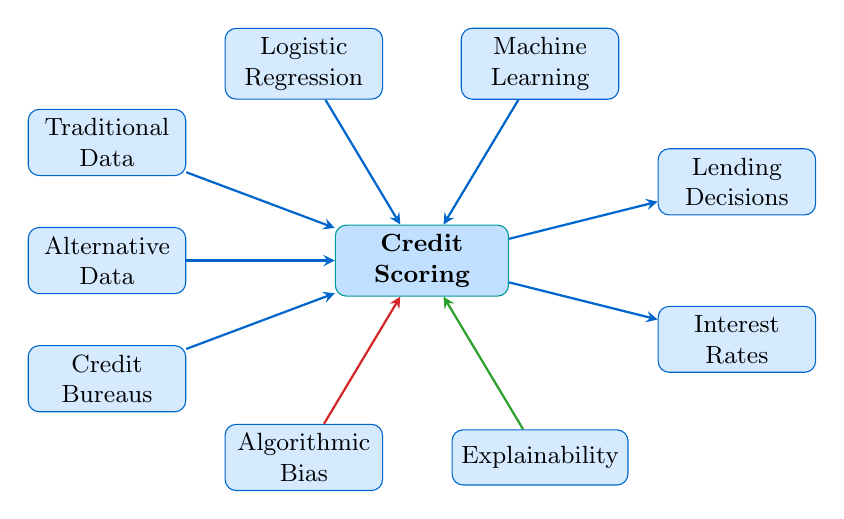
\begin{tikzpicture}[
    node distance=1.5cm,
    every node/.style={font=\small},
    box/.style={rectangle, rounded corners, draw=dfblue, fill=dflightblue4, minimum width=2cm, minimum height=0.7cm, align=center},
    bigbox/.style={rectangle, rounded corners, draw=dfteal, fill=dflightblue3, minimum width=2.2cm, minimum height=0.8cm, align=center, font=\small\bfseries}
]

% Central node
\node[bigbox] (credit) at (0,0) {Credit\\Scoring};

% Data inputs (left)
\node[box] (trad) at (-4,1.5) {Traditional\\Data};
\node[box] (alt) at (-4,0) {Alternative\\Data};
\node[box] (bureau) at (-4,-1.5) {Credit\\Bureaus};

% Model types (top)
\node[box] (logreg) at (-1.5,2.5) {Logistic\\Regression};
\node[box] (ml) at (1.5,2.5) {Machine\\Learning};

% Outputs (right)
\node[box] (decision) at (4,1) {Lending\\Decisions};
\node[box] (price) at (4,-1) {Interest\\Rates};

% Constraints (bottom)
\node[box] (bias) at (-1.5,-2.5) {Algorithmic\\Bias};
\node[box] (explain) at (1.5,-2.5) {Explainability};

% Arrows
\draw[arrow] (trad) -- (credit);
\draw[arrow] (alt) -- (credit);
\draw[arrow] (bureau) -- (credit);
\draw[arrow] (logreg) -- (credit);
\draw[arrow] (ml) -- (credit);
\draw[arrow] (credit) -- (decision);
\draw[arrow] (credit) -- (price);
\draw[arrow, dfred] (bias) -- (credit);
\draw[arrow, dfgreen] (explain) -- (credit);

\end{tikzpicture}
\end{center}

\vspace{2mm}
\textcolor{dfred}{Red}: Constrains/challenges \quad \textcolor{dfgreen}{Green}: Enables/improves
\end{frame}

% ============================================================================
% SLIDE 33: Key Terms & Definitions (Part 1)
% ============================================================================
\begin{frame}{Key Terms \& Definitions (1/2)}
\begin{description}
\item[Credit Score] A numerical summary of creditworthiness, predicting probability of default. FICO range: 300--850.

\item[Credit Bureau] Organizations (Equifax, Experian, TransUnion) that collect and sell credit data to lenders.

\item[Alternative Data] Non-traditional information (bank transactions, rent, utilities) used to assess creditworthiness.

\item[Thin-File Borrower] Individual with insufficient traditional credit history to generate a conventional score.

\item[Credit Invisible] Person with no credit file at bureaus---approximately 45 million Americans.
\end{description}
\end{frame}

% ============================================================================
% SLIDE 34: Key Terms & Definitions (Part 2)
% ============================================================================
\begin{frame}{Key Terms \& Definitions (2/2)}
\begin{description}
\item[Disparate Impact] When neutral policies disproportionately harm protected groups, even without intent.

\item[Adverse Action Notice] Required explanation when credit is denied, must cite specific reasons.

\item[SHAP Values] Technique to explain how each feature contributes to an individual prediction.

\item[AUC/Gini] Model evaluation metrics measuring ability to rank-order risk correctly.

\item[Reject Inference] The problem of not knowing outcomes for rejected applicants---creates selection bias.
\end{description}

\vspace{3mm}
\textbf{Tip}: Understanding these terms is essential for both building and auditing credit models.
\end{frame}

% ============================================================================
% SLIDE 35: Common Misconceptions
% ============================================================================
\begin{frame}{Common Misconceptions: Myth vs. Reality}
\begin{columns}[T]
\begin{column}{0.5\textwidth}
\begin{alertblock}{Myth 1}
``My credit score is a single, universal number.''
\end{alertblock}
\textbf{Reality}: You have multiple scores---FICO has 28 versions, plus VantageScore and lender-specific models.

\vspace{3mm}
\begin{alertblock}{Myth 2}
``Checking my own credit hurts my score.''
\end{alertblock}
\textbf{Reality}: Soft inquiries (checking your own score) have no impact. Only hard inquiries from applications affect scores.
\end{column}
\begin{column}{0.5\textwidth}
\begin{alertblock}{Myth 3}
``ML models are automatically fair because they're objective.''
\end{alertblock}
\textbf{Reality}: Models learn from historical data that may contain discrimination. Bias in = bias out.

\vspace{3mm}
\begin{alertblock}{Myth 4}
``Alternative data only helps FinTechs.''
\end{alertblock}
\textbf{Reality}: Incumbents like Experian (Boost) and FICO (XD) are incorporating alternative data too.
\end{column}
\end{columns}
\end{frame}

% ============================================================================
% SLIDE 36: Self-Assessment Questions (1/2)
% ============================================================================
\begin{frame}{Self-Assessment: Test Your Understanding (1/2)}
\begin{block}{Question 1 (Easy)}
What is the primary purpose of a credit scoring model?
\begin{enumerate}[A)]
\item To estimate the probability that a borrower will default on a loan
\item To calculate the exact amount a borrower can afford to repay
\item To determine the optimal interest rate for any loan
\item To track a borrower's payment history over time
\end{enumerate}
\end{block}

\vspace{2mm}
\pause
\textbf{Answer: A}---Credit scoring models estimate default probability. While this influences amounts and rates, the core purpose is probability estimation of repayment failure.

\vspace{4mm}
\begin{block}{Question 2 (Medium)}
How are scorecard points typically calculated in traditional credit scoring?
\begin{enumerate}[A)]
\item By multiplying feature values by their coefficients and scaling to a point system
\item By counting the number of positive features and subtracting negative ones
\end{enumerate}
\end{block}
\pause
\textbf{Answer: A}---Points derive from logistic regression coefficients, scaled to an intuitive range.
\end{frame}

% ============================================================================
% SLIDE 37: Self-Assessment Questions (2/2)
% ============================================================================
\begin{frame}{Self-Assessment: Test Your Understanding (2/2)}
\begin{block}{Question 3 (Hard)}
What is the difference between ``through-the-door'' and ``clean-sample'' model development?
\begin{enumerate}[A)]
\item Through-the-door uses all applicants; clean-sample excludes rejected applicants
\item Through-the-door is for online applications; clean-sample is for in-branch
\item Through-the-door includes alternative data; clean-sample uses only traditional data
\item Through-the-door is for new customers; clean-sample is for existing customers
\end{enumerate}
\end{block}

\vspace{2mm}
\pause
\textbf{Answer: A}---Through-the-door development attempts to use all applicants (handling reject inference), while clean-sample uses only approved applicants with observed outcomes. Clean-sample is simpler but suffers from selection bias.

\vspace{4mm}
\textbf{Reflection}: Can you explain why selection bias matters for model accuracy?
\end{frame}

% ============================================================================
% SLIDE 38: What's Next
% ============================================================================
\begin{frame}{What's Next: Topic 2.4 -- Platform Economics}
\begin{columns}[T]
\begin{column}{0.5\textwidth}
\textbf{Preview: Platform Economics}
\begin{itemize}
\item Network effects in FinTech
\item Two-sided marketplaces
\item Winner-take-most dynamics
\item Platform vs. pipeline business models
\end{itemize}

\vspace{3mm}
\textbf{Key Question}: Understanding which FinTech innovations are sustainable vs. venture-subsidized.
\end{column}
\begin{column}{0.5\textwidth}
\begin{block}{Connection to This Topic}
\begin{itemize}
\item Data flywheel creates platform advantages
\item Lending marketplaces use network effects
\item Data network effects compound over time
\item Platform economics explains FinTech valuations
\end{itemize}
\end{block}

\vspace{2mm}
\textbf{Preparation}: Think about platforms you use---what makes them ``sticky''?
\end{column}
\end{columns}
\end{frame}

% ============================================================================
% SLIDE 39: Resources
% ============================================================================
\begin{frame}{Resources for Further Learning}
\begin{columns}[T]
\begin{column}{0.5\textwidth}
\textbf{Academic Papers:}
\begin{itemize}
\item Fuster et al. (2022): ``Predictably Unequal?''---ML and mortgage lending
\item Bartlett et al. (2022): ``Consumer Lending Discrimination''
\item Kleinberg et al. (2018): ``Discrimination in Age of Algorithms''
\end{itemize}

\vspace{3mm}
\textbf{Industry Reports:}
\begin{itemize}
\item CFPB: ``Big Data'' reports
\item Federal Reserve: ``Alternative Data'' analysis
\item Brookings: Financial inclusion studies
\end{itemize}
\end{column}
\begin{column}{0.5\textwidth}
\textbf{Books:}
\begin{itemize}
\item \textit{Weapons of Math Destruction} (O'Neil)
\item \textit{The Credit Scoring Toolkit} (Anderson)
\item \textit{Automating Inequality} (Eubanks)
\end{itemize}

\vspace{3mm}
\textbf{Online Tools:}
\begin{itemize}
\item AnnualCreditReport.com (free reports)
\item SHAP library documentation
\item Kaggle: Credit scoring datasets
\end{itemize}

\vspace{3mm}
\textbf{Regulatory:}
\begin{itemize}
\item ECOA, FCRA, GDPR texts
\item EU AI Act (credit = high-risk)
\end{itemize}
\end{column}
\end{columns}
\end{frame}

% ============================================================================
% SLIDE 40: Questions
% ============================================================================
\begin{frame}
\centering
\vspace{15mm}
{\Huge\textbf{Questions?}}

\vspace{10mm}
\textbf{Topic 2.3: Data-Driven Finance}\\
\textit{Lending, Scoring, and Algorithmic Decision-Making}

\vspace{10mm}
\begin{block}{}
\centering
Joerg Osterrieder\\
Digital Finance\\
\texttt{joerg.osterrieder@ifi.uzh.ch}
\end{block}

\vspace{5mm}
\textbf{Next Up}: Topic 2.4 -- Platform Economics
\end{frame}

\end{document}
